\section{Research}
First a list of available information that can be achieved from the
mesurement:
\begin{itemize}
  \item the glucose level
  \item the time difference between now and the previous injections
  \item the gradient of the glucose curve at the time of the current measurement
  \item the insulin that will be available in the period p which can be
  calculated as now + ``length of p'' (p can be e.g. 1, 2, 5, 10, 30, \ldots
  minutes or 1, 2, 5, 10, \ldots hours)
  \item the average of the glucose level since a defined point t in the past (t
  has the same definition as p)
\end{itemize}

\subsection{Calculation steps}
\subsubsection{Calculate the gradient (GR) for the current timestamp}
Because of the reason that we don’t have the function of the glucose curve so
that we can derive from we need to calculate the gradient.
One way is to take the gradient from the last and the actual measurement.

\subsubsection{Calculate the available insulin (IN)}
The available insulin can be calculates like in the simulation that you take
the actual timestamp and simply add a period to this time. With the new
timestamp the module insulin and rhe module pangria can calculate the available
insulin for a given period in the future.

\subsubsection{Calculate the actual needed amount of insulin}
As higher GR is as longer the insulin level would increase. Then much more
insulin is needed to get the level down to normal. Than we can calculate with
the amount that is needed to get the glucose level to normal and subtract IN
from this. The result (RE) can be injected.
This is a very simple attempt to calculate the needed amount of insulin.

I assume that we can set a static amount of insulin that will be given by the
pangria. This static amount will be included in the calculation.

\subsection{Further Thoughts}
\begin{itemize}
  \item it is possible to put an factor in front of RE so that just a part of
  the insulin will be injected. The factor depends on GR
  \item we should think about the time period between the measurements to the
  best result
  \item we should define some levels where we put some extra insulin the avoid
  peaks e.g. if we have a big GR but we where in the dangerous area of to less
  sugar then it so problem but if we are in an area where we are already to
  high than is very dangerous
  \item it is possible not to calculate the amount for the future but for the
  past so that we say in the last period the amount of glucose is increased  by
  ``x'' how much insulin is needed to absorb the glucose
  \item in some way we should have a warning in the pump where we inform the
  user if he is in the dangerous area (to high or to low)
\end{itemize}

\section{Analysis Model}

\subsection{Automation of the Insulin pump}
In the first step we divided our glucose range in 4 different. These parts are already mentioned in the research part.

Critical to low level (LL) – glucose level is less or equal to 4 mmol/l

Normal  level (NL) - glucose level between 4 and 7,5 mmol/l

Increased level (IL) - glucose level between 7,5 and 10 mmol/l

Critical to high level (HL) - glucose level is equal or greater than 4 mmol/l

\subsubsection{The measuring process}
For the measurement we decided to use the following values:
\begin{itemize}
  \item Difference in the glucose level between either the last injection or
  the point in time where the level reaches the increased level coming from the normal level.
  \item The insulin that will be available in a defined period (e.g. 3h) 
\end{itemize}

\subsubsection{The calculation}
There are two values that need to be calculated
\begin{itemize}
  \item The time between the injections
  \item The amount of insulin that will be injected  
\end{itemize}
These two values can be either fixed or dynamic. In the following Paragraphs all combinations will be discussed.

\paragraph{Fixed amount of insulin and fixed time difference}
This is a pretty simple idea which comes from the fact that if a person is ill the pump could keep person on a constant healthy insulin level. A problem is that this attempt can’t react on peaks in the glucose level. So this is to less.

\paragraph{Dynamic amount of insulin and fixed time difference}
In this attempt there is an algorithm where we calculate a factor from the difference in the glucose level between 2 measurements.
\begin{figure}[htb]
\centering
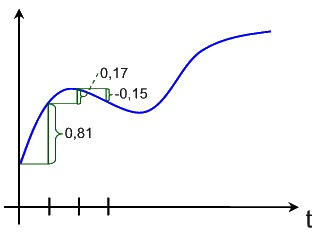
\includegraphics[width=\textwidth]{images/graf1.jpg}
\caption{Formula 1}
\label{fig:formula_1}
\end{figure}
This factor (F) then can be multiplied with a fixed an predefined amount of insulin (I). The injection just happens if the factor is positive. This is an attempt which gives a first result where the peeks are handled. The problem is after the peek there is a hangover of the effect of insulin so that the glucose level is falling down maybe to the LL which can end up in a clops or dead.

\paragraph{Fixed amount of insulin and dynamic time difference}
In this attempt we have small periods (e.g. 30s) between the measurements. If the difference in the glucose level between the current measurement and the last injection, exceeds a defined factor than a fixed amount of insulin will be injected.
\begin{figure}[htb]
\centering
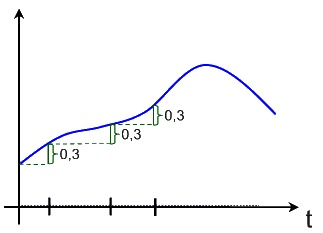
\includegraphics[width=\textwidth]{images/graf2.jpg}
\caption{Formula 2}
\label{fig:formula_2}
\end{figure}
In this attempt the there is the same problem with the hangover of the effect of al the injections as it was in the attempt before.

\paragraph{Dynamic amount of insulin and dynamic time difference}
To handle all the problems which have been mentioned we need both ideas combined together. The following steps are needed in this algorithm:
\begin{itemize}
  \item First thing is to define a so called reference level (RL) wich will be
  somewhere in the middle of the normal level range
  \item For the different levels we have different factors which need to be
  reached. These factors are calculated from the difference since the last injection or the last entrance of the increased level for the increased and the tor high level there are different factors so that if the to high level is reached the period between the injections will be shorter.
  \item If the factor is reached the amount of insulin will be calculated.
  \item First the available amount of insulin (AI = Available insulin) can be
  calculated by the insulin-module with the information of the preceding injections and by the pangria-module.
  \item With this information we can calculate the amount of glucose that will
  be absorbed (AG = Absorbed glucose) by the insulin
  \item now we can calculate the difference between the actual glucose level
  (AGL = Actual Glucose Level) and the RL. There we get the needed Insulin (NI = Needed Insulin).
  \item From this it follows that we have the difference (GD = Glucose
  difference) between the AGL and the AG
  \item After that we can calculate the insulin level for GD and inject it.
\end{itemize}

\begin{figure}[htb]
\centering
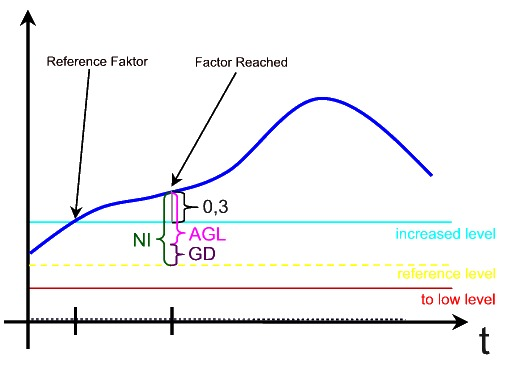
\includegraphics[width=\textwidth]{images/graf3.jpg}
\caption{Formula 3}
\label{fig:formula_3}
\end{figure}
This algorithm should hold the glucose level in average on a normal level.

\section{Design Model}
Thanks to the very open and felxible implementation of the Body Simulation
following the Model View Controller (see section \vref{sec:body_simulation})
paradigm, the sensor and injector components of the Insulin pump can be very
easily integrated into the model.

\begin{figure}[htb]
\centering
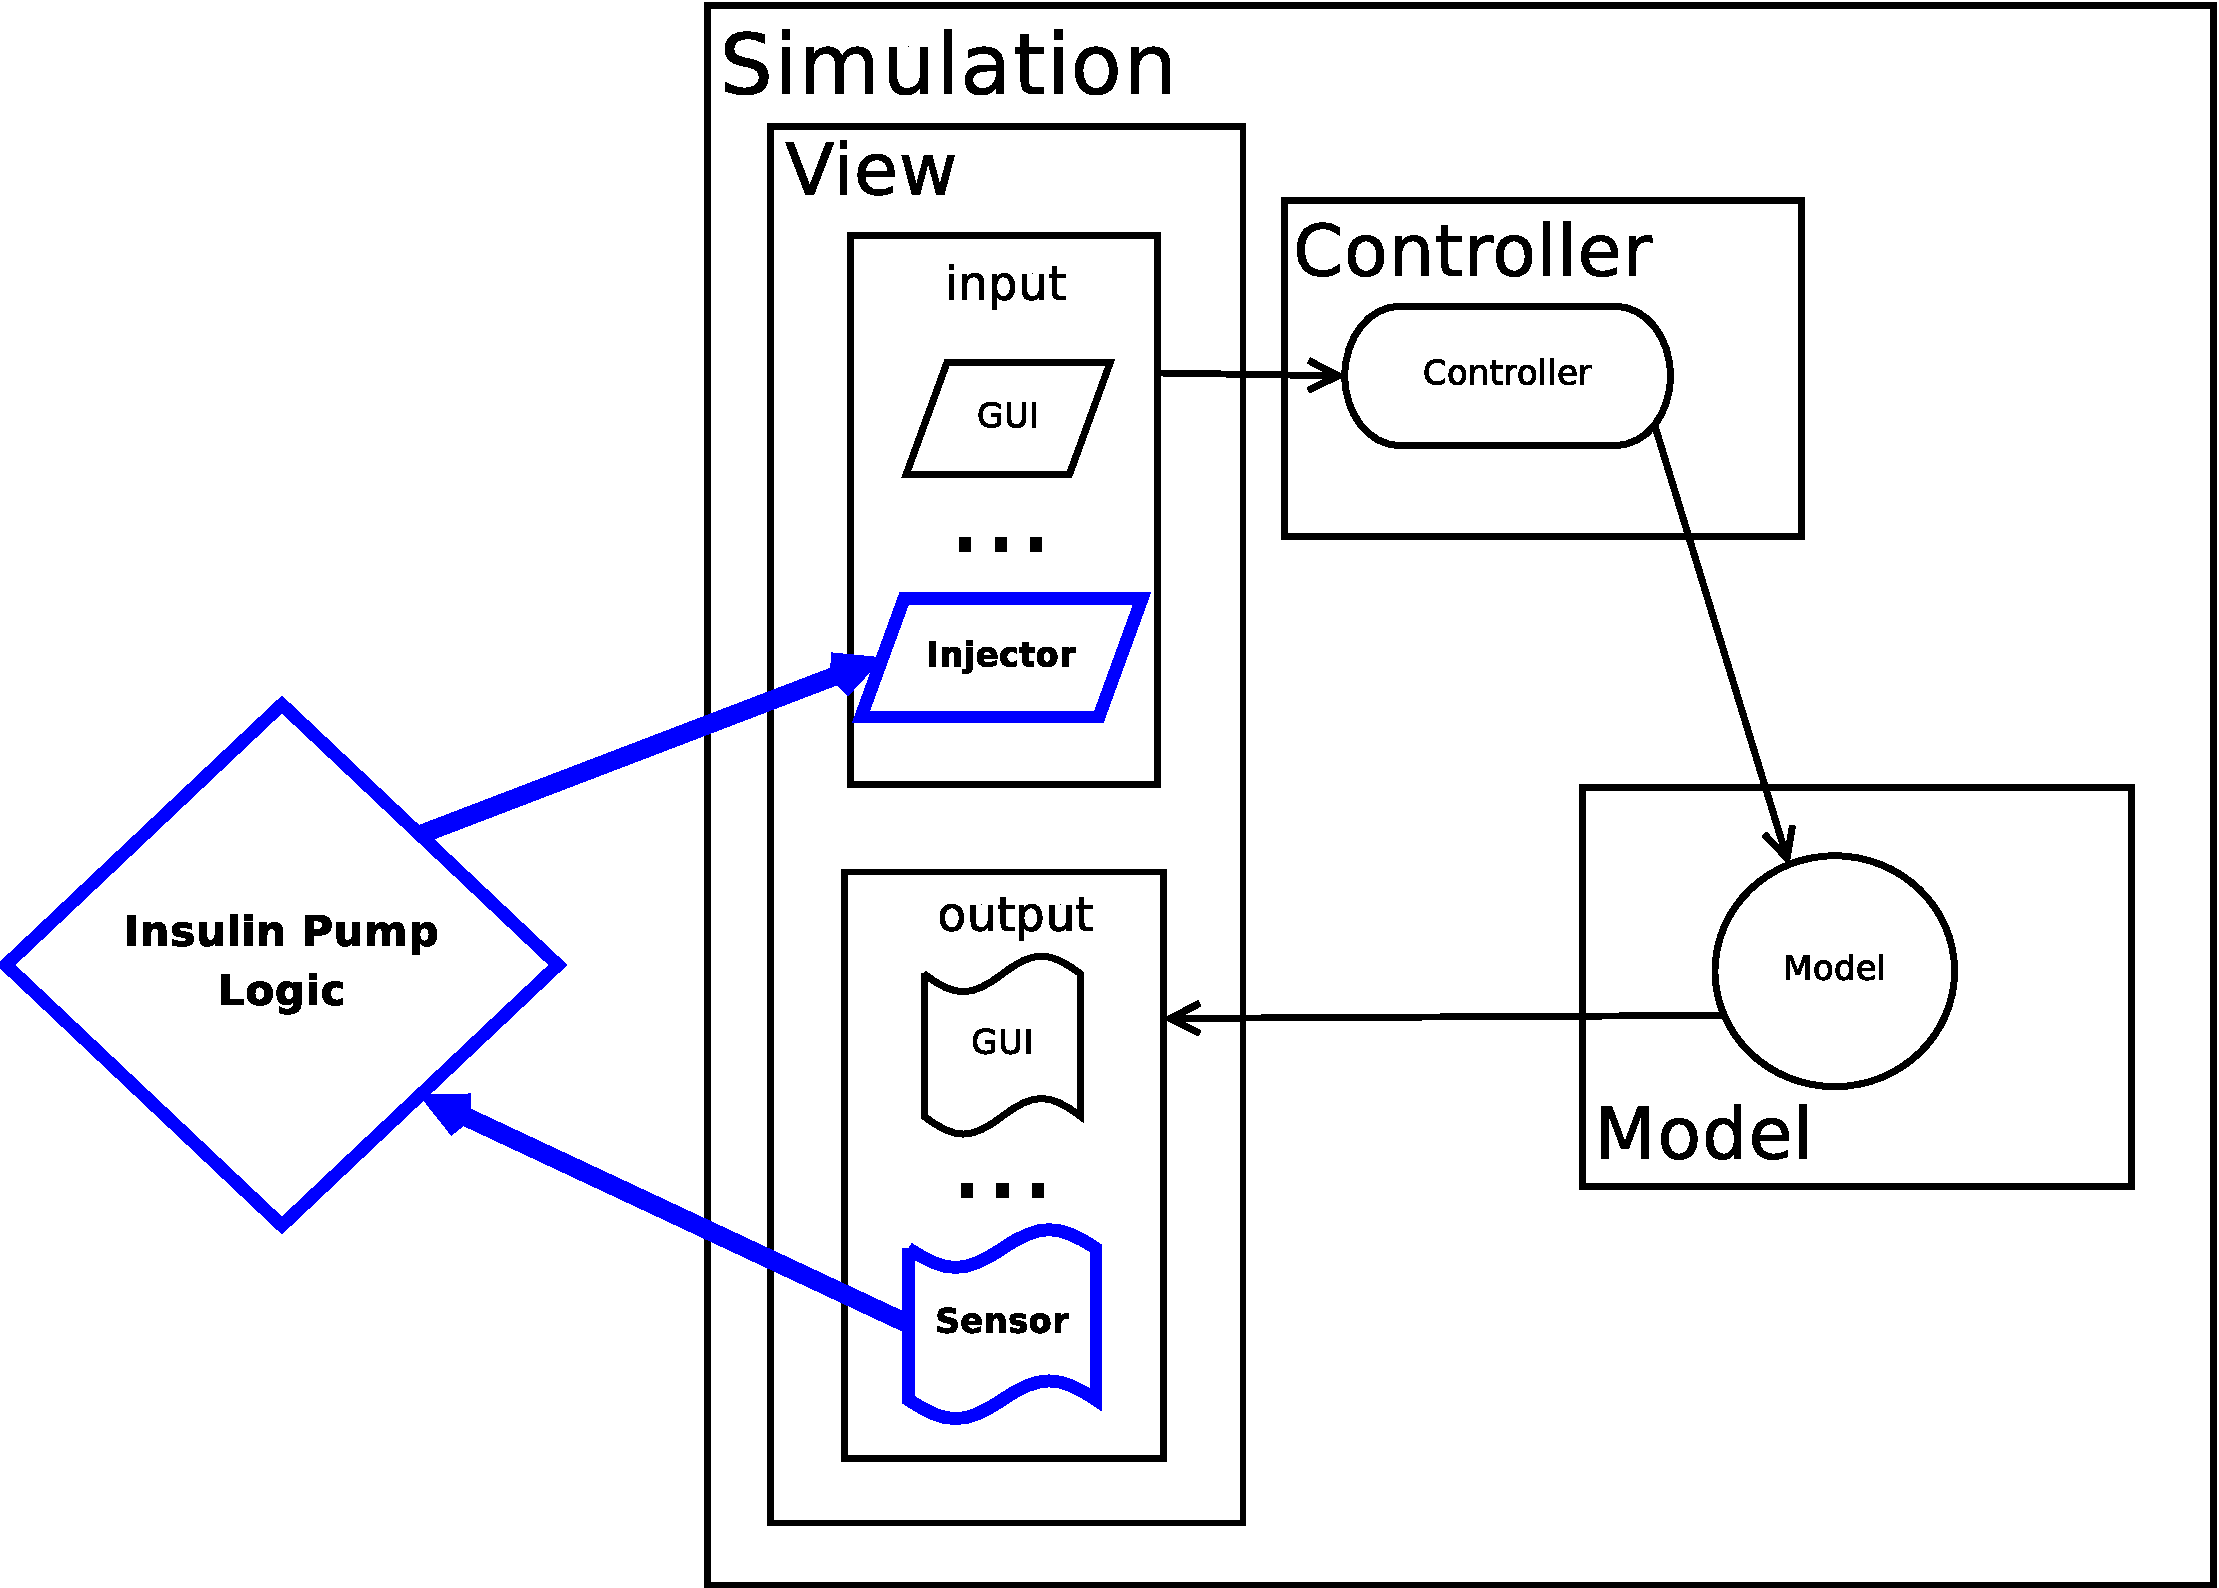
\includegraphics[scale=0.39]{images/mvc_insulin_pump}
\caption{Integration of the Insulin Pump into the Body Simulation}
\label{fig:mvc_insulin_pump}
\end{figure}
